\documentclass[10pt,aspectratio=169]{beamer}

\usepackage[utf8x]{inputenc}
\usepackage[T1]{fontenc}
\usepackage{lmodern}

\usepackage{amsmath,amssymb,mathtools}
\usepackage{bm}
\usepackage{cancel}
\usepackage{empheq}
\usepackage{graphicx}
\usepackage{array,booktabs,tabularx,tabulary,multirow}
\usepackage{tikz}
\usepackage{hyperref}
\usepackage{feynmp}

\newcolumntype{V}{>{\centering\arraybackslash} m{.2\linewidth} }

\usetikzlibrary{arrows,matrix,shapes,positioning}
\usetikzlibrary{calc}
\usetikzlibrary{mindmap}
\usetikzlibrary{shadows.blur}

\newcommand*\widefbox[1]{\fbox{\hspace{0.5em}#1\hspace{0.5em}}}
\newcommand{\DRbar}{{\overline{\textrm{DR}}}}
\newcommand{\SUSYv}{{\cancel{SUSY}}}

\DeclareMathOperator{\Tr}{Tr}
\DeclareMathOperator{\STr}{STr}

\DeclareGraphicsRule{*}{mps}{*}{}
\graphicspath{{./figures/}}

\title{Dark Matter Predictions in $E_6$ Inspired SUSY Models}

\author{D.~Harries\\
  {\scriptsize
  (IPNP, Charles University in Prague)}
  }

\titlegraphic{
  \begin{center}
    \hspace*{\fill}
    
\includegraphics[scale=0.3]{uk_logo}
    \hspace*{\fill}
  \end{center}
}

\date[\'{U}TF, Charles University in Prague]{April 9, 2018}

\usetheme{CambridgeUS}

\setbeamertemplate{headline}[default]{}
\setbeamertemplate{footline}[page number]{}
\setbeamertemplate{navigation symbols}{}

\begin{document}

\begin{frame}[plain]
  \titlepage
\end{frame}

\section{Motivation}

\begin{frame}
  \frametitle{Evidence for DM}
  \begin{columns}[t]
    \begin{column}{0.3\textwidth}
      \vspace*{-20pt}
      \begin{figure}
        \centering
        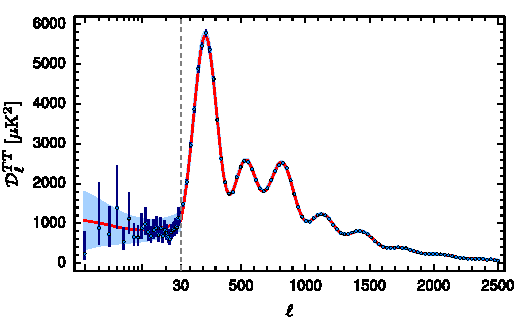
\includegraphics[width=0.95\textwidth]{cmb_power_spectrum}
      \end{figure}
      \vspace*{-25pt}
      \begin{center}
        { \tiny [\href{http://arxiv.org/abs/1502.02114}{%
              arXiv:1502.02114}] }
      \end{center}
      \vspace*{-20pt}
      \begin{center}
        CMB measurements
      \end{center}
      \vspace*{-15pt}
      \begin{figure}
        \centering
        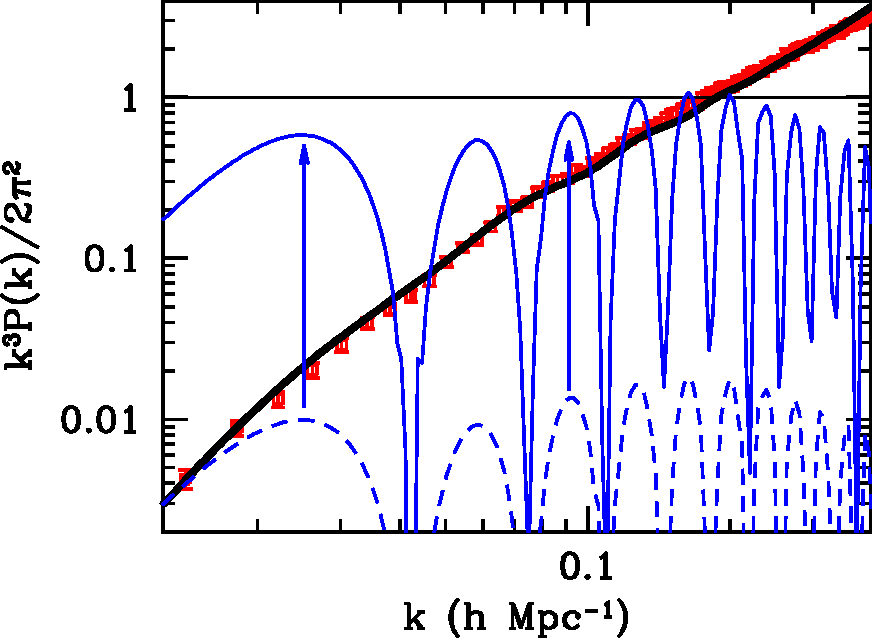
\includegraphics[width=0.95\textwidth]{matter_power_spectrum}
      \end{figure}
      \vspace*{-20pt}
      \begin{center}
        { \tiny [\href{http://arxiv.org/abs/1112.1320}{%
              arXiv:1112.1320}] }
      \end{center}
      \vspace*{-20pt}
      \begin{center}
        Structure formation
      \end{center}
    \end{column}
    \begin{column}{0.3\textwidth}
      \begin{figure}
        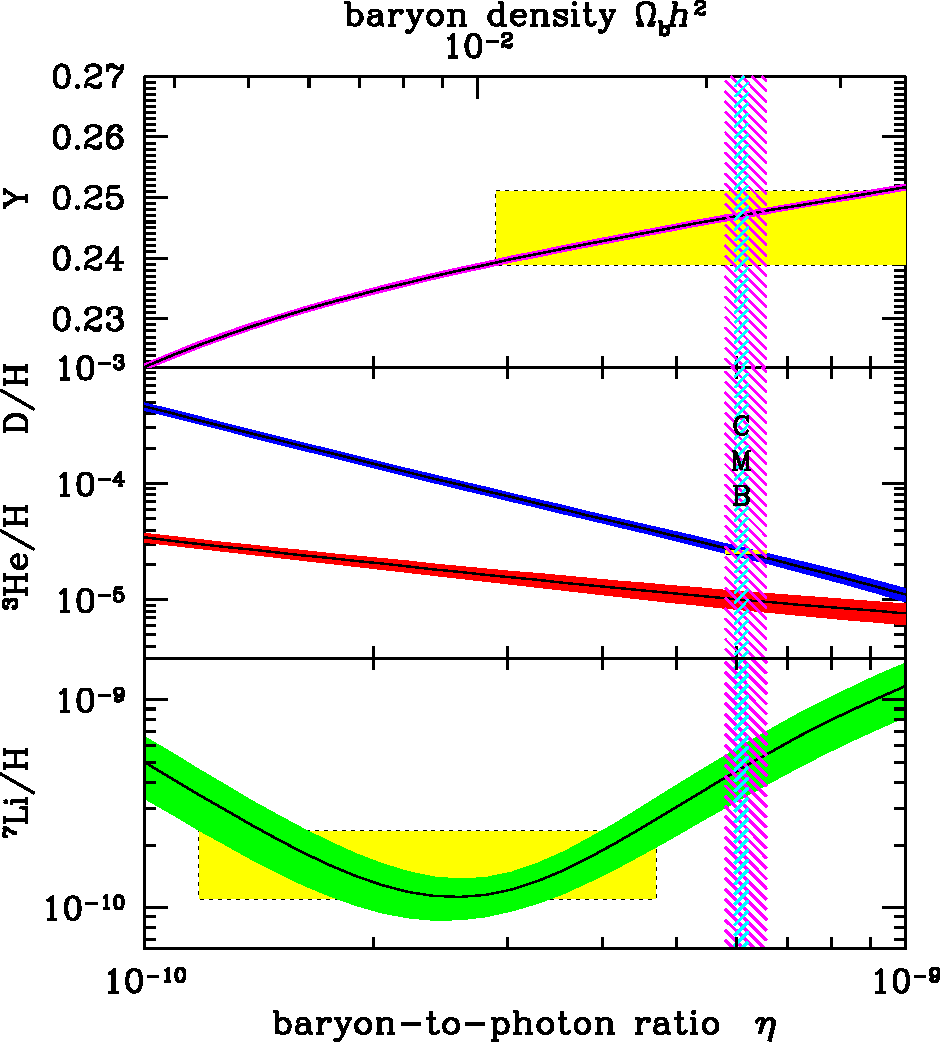
\includegraphics[width=\textwidth]{bbn}
      \end{figure}
      \vspace*{-25pt}
      \begin{center}
        { \tiny [\href{http://pdg.lbl.gov/2017/reviews/rpp2017-rev-bbang-nucleosynthesis.pdf}{%
              PDG 2017}] }
      \end{center}
      \vspace*{-15pt}
      \begin{center}
        BBN
      \end{center}
    \end{column}
    \begin{column}{0.3\textwidth}
      \vspace*{-20pt}
      \begin{figure}
        \centering
        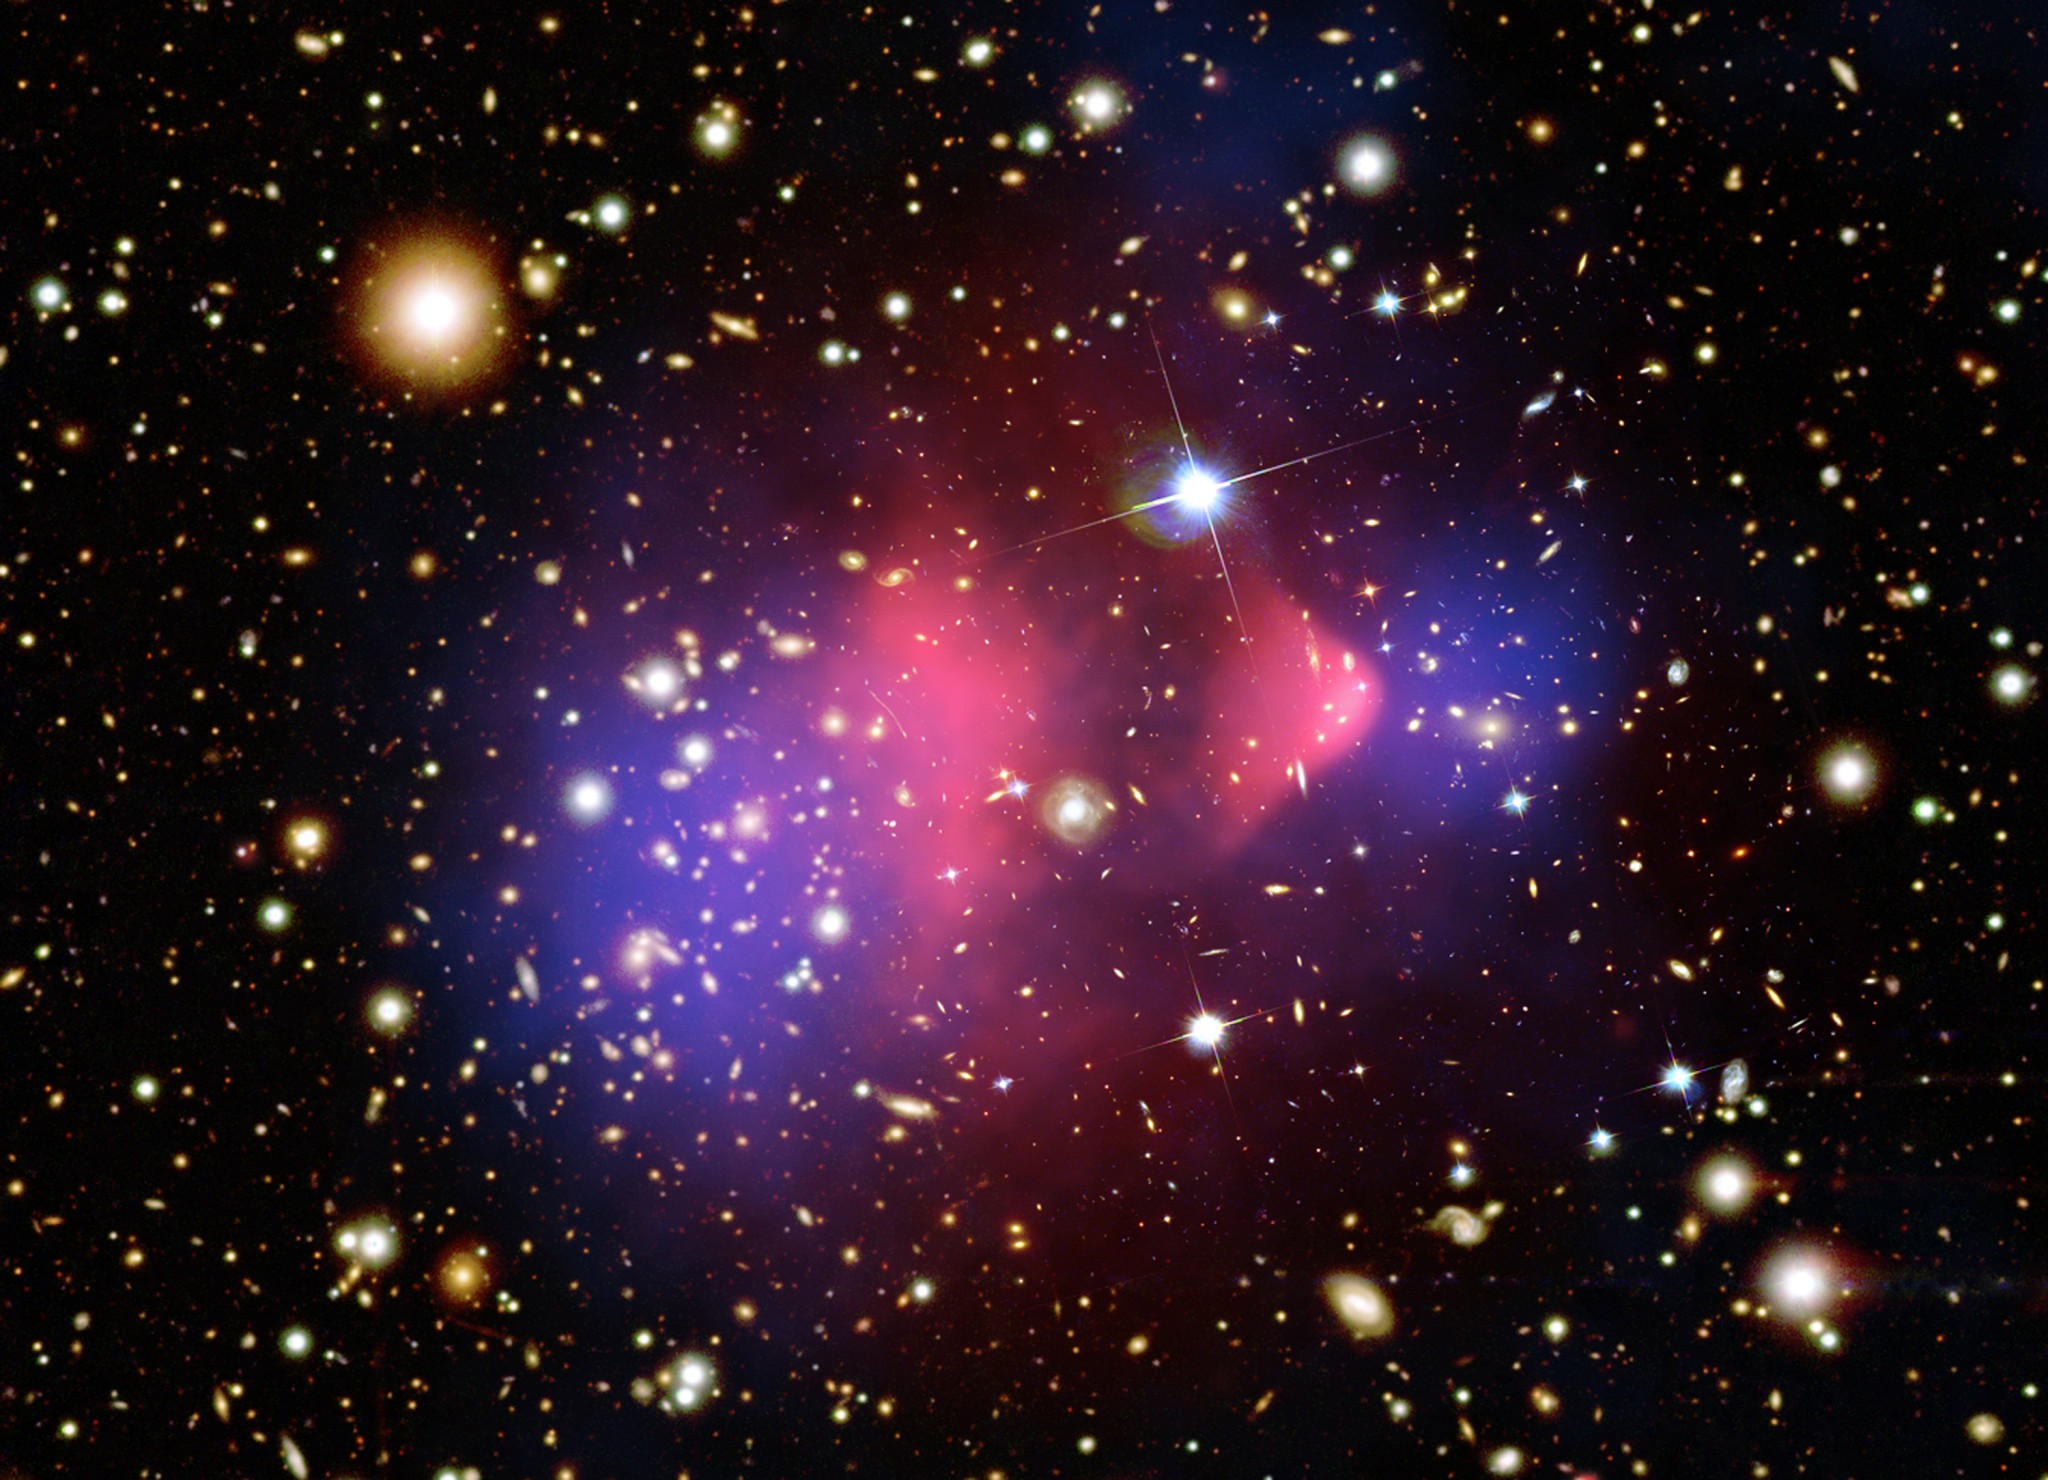
\includegraphics[width=0.85\textwidth]{bulletcluster}
      \end{figure}
      \vspace*{-25pt}
      \begin{center}
        {\tiny [\href{https://apod.nasa.gov/apod/ap060824.html}{APOD/NASA}]}
      \end{center}
      \vspace*{-20pt}
      \begin{center}
        Galaxy cluster mergers
      \end{center}
      \vspace*{-10pt}
      \begin{figure}
        \centering
        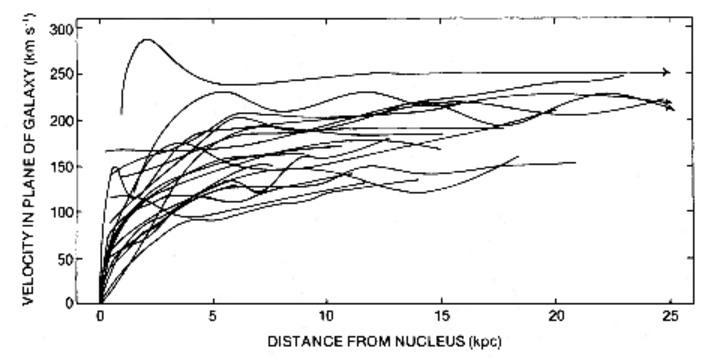
\includegraphics[width=\textwidth]{rotation_curves}
      \end{figure}
      \vspace*{-25pt}
      \begin{center}
        { \tiny [V.~C.~Rubin, N.~Thonnard, and W.~K.~Ford, Jr.,
            \href{http://doi.org/10.1086/158003}{%
              Astrophys.~J.~\textbf{238} (1980) 471}] }
      \end{center}
      \vspace*{-17pt}
      \begin{center}
        Galaxy rotation curves
      \end{center}
    \end{column}
  \end{columns}
\end{frame}

\begin{frame}
  \frametitle{DM Candidates}
  \begin{figure}
    \centering
    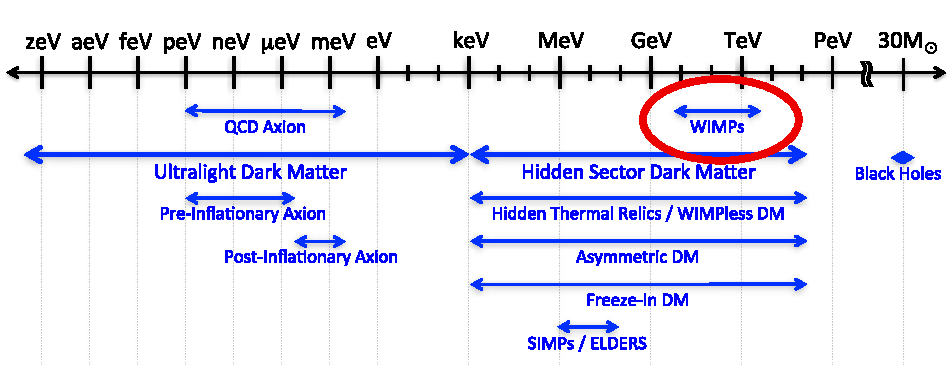
\includegraphics[width=\textwidth]{dmcandidates}
  \end{figure}
  \vspace*{-20pt}
  \begin{center}
    {\tiny [\href{http://arxiv.org/abs/1707.04591}{%
          arXiv:1707.04591}]}
  \end{center}
\end{frame}

\begin{frame}
  \frametitle{WIMP DM: Relic Density}
  \begin{columns}[t]
    \begin{column}{0.5\textwidth}
      \begin{itemize} \itemsep1em
      \item Relic density of standard WIMPs results from
        freeze-out ($Y = n_\chi / s$),
        \begin{equation*}
          \frac{d Y}{d t} = - s \langle \sigma v \rangle ( Y^2
          - Y^2_{\text{eq.}} )
          \Rightarrow
          \Omega_\chi h^2 = \frac{m_\chi s_0 h^2}{\rho_c} Y_\infty
        \end{equation*}
      \item ``WIMP miracle'': for $m_\chi \sim$ GeV $-$ TeV,
        $g_\chi \sim g_{\text{weak}}$,
        \begin{equation*}
          \Omega_\chi \sim \frac{m_\chi^2}{g_\chi^4} \sim \Omega_{\text{DM}}
        \end{equation*}
      \item \alert{$\Omega_\chi h^2 > (\Omega_{\text{DM}} h^2)_{\text{Planck}}$
        $\Rightarrow$ model ruled out}
        \begin{itemize} \itemsep0.5em
        \item N.B. $\Omega_\chi h^2 < (\Omega_{\text{DM}} h^2)_{\text{Planck}}$
          allowed
        \item e.g., multiple DM candidates $\chi_i$, $\sum_i \Omega_{\chi_i} =
          \Omega_{\text{DM}}$
        \end{itemize}
      \end{itemize}
    \end{column}
    \begin{column}{0.5\textwidth}
      \vspace*{-20pt}
      \begin{figure}
        \centering
        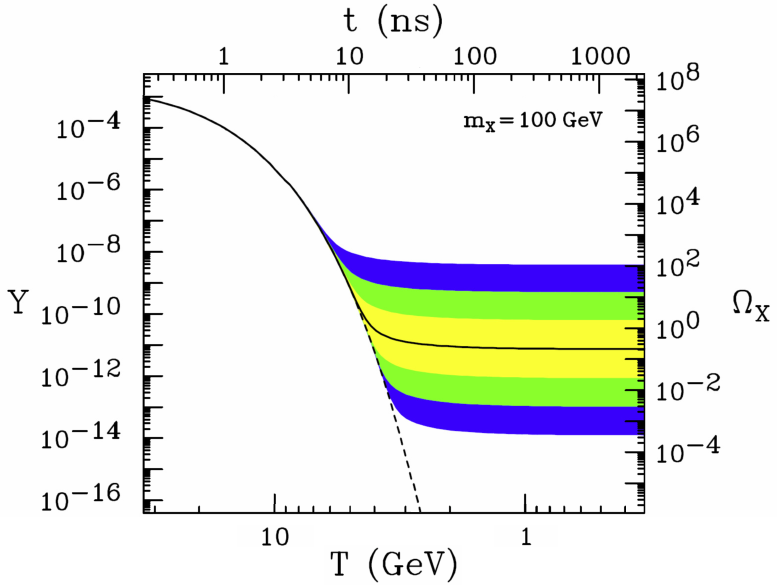
\includegraphics[width=\textwidth]{freezeout}
      \end{figure}
      \vspace*{-20pt}
      \begin{center}
        { \tiny [\href{http://arxiv.org/abs/1003.0904}{%
              arXiv:1003.0904}] }
      \end{center}
      \begin{center}
        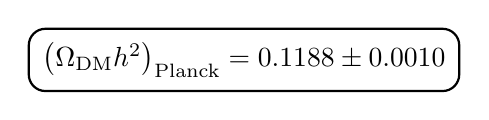
\begin{tikzpicture}
          \node[rectangle, draw, fill = white, rounded corners = 6pt,
          thick, inner sep = 0.5em]{%
            $\left ( \Omega_{\text{DM}} h^2 \right )_{\text{Planck}}
            = 0.1188 \pm 0.0010$
          };
        \end{tikzpicture}
      \end{center}
    \end{column}
  \end{columns}
\end{frame}

\begin{frame}
  \frametitle{Constraining WIMP Models}
  \begin{columns}[t]
    \begin{column}{0.5\textwidth}
      \begin{figure}
        \centering
        \includegraphics[height=0.4\textwidth]{dmsignals}
      \end{figure}
      \vspace*{-10pt}
      \begin{itemize} \itemsep1em
      \item Multiple approaches: {\color{blue} direct detection}
        ($\rightarrow$), indirect detection ($\uparrow$), collider searches
        ($\downarrow$)
      \item Direct detection: observe nuclear recoil in DM-nucleus interaction,
        \begin{equation*}
          \frac{d R}{d E} =\frac{1}{2 m_\chi m_r^2} {\color{red}
            \sigma(q) \rho_{\chi, \text{local}}} \eta(v_{\text{min}}(E), t)
        \end{equation*}
      \end{itemize}
    \end{column}
    \begin{column}{0.5\textwidth}
      \begin{itemize}\itemsep1em
      \item \alert{LUX, XENON1T, $\ldots$ $\Rightarrow$ stringent limits on
        $\sigma^{(SI/SD)}$:}
      \end{itemize}
      \begin{figure}
        \centering
        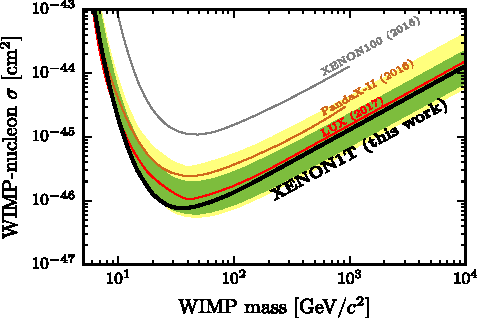
\includegraphics[width=\textwidth]{xenon1t_si_limit}
      \end{figure}
      \vspace*{-20pt}
      \begin{center}
        {\tiny [\href{http://arxiv.org/abs/1705.06655}{%
              arXiv:1705.06655}]}
      \end{center}
    \end{column}
  \end{columns}
\end{frame}

\begin{frame}
  \frametitle{The MSSM}
  \begin{columns}
        \begin{column}{0.5\textwidth}
      \begin{figure}
        \centering
        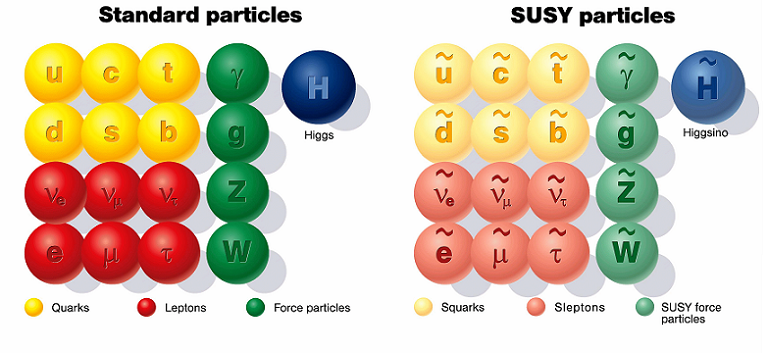
\includegraphics[width=\textwidth]{susyparticles_sm}
      \end{figure}
      \vspace*{-20pt}
      \begin{center}
        {\tiny [\href{http://www.physics.gla.ac.uk/ppt/bsm.htm}{%
      http://www.physics.gla.ac.uk/ppt/bsm.htm}] }
      \end{center}
    \end{column}
    \begin{column}{0.5\textwidth}
      \begin{table}[h]
        \centering
        \scriptsize
        \begin{tabular}{cccccc}
          \toprule
          $\hat{\Phi}$ & $s = 0$ & $s = \frac{1}{2}$ & $SU(3)_C$ & $SU(2)_L$
          & $\sqrt{\frac{5}{3}} Q_i^Y$ \\
          \midrule
          $\hat{Q}_i$ & $\begin{pmatrix} \tilde{u}_{L} \\
            \tilde{d}_{L} \end{pmatrix}_i$
            & $\begin{pmatrix} u_{L} \\ d_L\end{pmatrix}_i$
            & $\mathbf{3}$ & $\mathbf{2}$ & $\frac{1}{6}$ \\[1em]
          $\hat{u}^c_i$ & $\tilde{u}^*_{iR}$ & $u^c_{iR}$
            & $\bar{\mathbf{3}}$ & $\mathbf{1}$ & $-\frac{2}{3}$ \\[0.5em]
          $\hat{d}^c_i$ & $\tilde{d}^*_{iR}$ & $d^c_{iR}$
            & $\bar{\mathbf{3}}$ & $\mathbf{1}$ & $\frac{1}{3}$ \\[0.5em]
          $\hat{L}_i$ & $\begin{pmatrix} \tilde{\nu}_{L} \\
              \tilde{e}_{L} \end{pmatrix}_i$
            & $\begin{pmatrix} \nu_{L}\\ e_L \end{pmatrix}_i$
            & $\mathbf{1}$ & $\mathbf{2}$ & $-\frac{1}{2}$ \\[1em]
          $\hat{e}^c_i$ & $\tilde{e}^*_{iR}$ & $e^c_{iR}$
            & $\mathbf{1}$ & $\mathbf{1}$ & $1$ \\[0.5em]
          $\hat{H}_d$ & $\begin{pmatrix} H_d^0 \\ H_d^- \end{pmatrix}$
            & $\begin{pmatrix} \tilde{H}_d^0 \\ \tilde{H}_d^- \end{pmatrix}$
            & $\mathbf{1}$ & $\mathbf{2}$ & $-\frac{1}{2}$ \\[1em]
          $\hat{H}_u$ & $\begin{pmatrix} H_u^+ \\ H_u^0 \end{pmatrix}$
            & $\begin{pmatrix} \tilde{H}_u^+ \\ \tilde{H}_u^0 \end{pmatrix}$
            & $\mathbf{1}$ & $\mathbf{2}$ & $\frac{1}{2}$ \\[1em]
            \bottomrule
        \end{tabular}
      \end{table}
    \end{column}
  \end{columns}
      \begin{empheq}[box=\widefbox]{align*}
        W_{\text{MSSM}} &= \mu ( \hat{H}_d \cdot \hat{H}_u )
        + y_{ij}^e \hat{e}^c_i ( \hat{L}_j \cdot \hat{H}_d )
        + y_{ij}^d \hat{d}^c_i ( \hat{Q}_j \cdot \hat{H}_d )
        + y_{ij}^u \hat{u}_i^c ( \hat{H}_u \cdot \hat{Q}_j ) \\
        & \quad {} {\color{red} - \epsilon_i \hat{L}_i \cdot \hat{H}_u
          + \frac{1}{2} \rho_{ijk} \hat{L}_i \cdot \hat{L}_j \hat{e}_k^c
          + \rho^\prime_{ijk} \hat{L}_i \cdot \hat{Q}_j \hat{d}_k^c
          + \frac{1}{2} \rho^{\prime\prime}_{ijk} \hat{u}_i^c
          \hat{d}_j^c \hat{d}_k^c }
      \end{empheq}
\end{frame}

\begin{frame}
  \frametitle{Neutralino DM}
  \begin{columns}[t]
    \begin{column}{0.5\textwidth}
      \begin{itemize} \itemsep1em
      \item Forbid $B$, $L$ violating interactions $\Rightarrow$
        impose {\color{blue} $R$-parity $\Leftrightarrow$
        matter parity}
        \begin{equation*}
          Z_2^R = (-1)^{3(B - L) + 2 s} , \quad
          Z_2^M = (-1)^{3 (B - L)}
        \end{equation*}
      \item $\Rightarrow$ lightest $R$-parity odd state (LSP) is
        {\color{blue} natural WIMP DM candidate} (provided $Q_{LSP} = 0$)
      \item Standard MSSM candidate is
        \begin{equation*}
          \tilde{\chi}_1^0 = N_{11} \tilde{H}_d^0 + N_{12} \tilde{H}_u^0
          + N_{13} \tilde{W}_3 + N_{14} \tilde{B}
        \end{equation*}
      \item Properties dependent on $m_{\tilde{\chi}_1^0}$, $N_{ij}$
        (i.e., $\mu$, soft breaking $M_1$, $M_2$)
      \end{itemize}
    \end{column}
    \begin{column}{0.5\textwidth}
      \begin{figure}
        \centering
        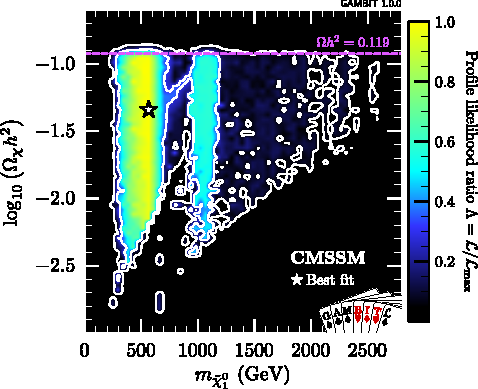
\includegraphics[width=0.9\textwidth]{gambit_gut_direct_detection}
      \end{figure}
      \vspace*{-20pt}
      \begin{center}
        { \tiny [\href{http://arxiv.org/abs/1705.07935}{%
              arXiv:1705.07935}] }
      \end{center}
    \end{column}
  \end{columns}
\end{frame}

\section{E$_6$ Inspired Models}

\begin{frame}
  \frametitle{E$_6$ Inspired Models}
  \begin{itemize} \itemsep1em
    \item Motivated by MSSM shortcomings, e.g., tree-level $m_{h_1}^2
      \leq M_Z^2 \cos^2 2\beta$ (\alert{``little hierarchy problem''}),
      \alert{$\mu$-problem}, $\nu$ masses, $\ldots$
    \item Lead to $U(1)$ extended models at low-energies:
      \begin{align*}
        E_6&\longrightarrow SO(10)\times U(1)_\psi \\
        &\longrightarrow SU(5)\times U(1)_\psi\times U(1)_\chi\\
        &\longrightarrow SU(3)_C\times SU(2)_L\times U(1)_Y\times
        U(1)_\psi\times U(1)_\chi\\
        &\longrightarrow SU(3)_C\times SU(2)_L\times U(1)_Y\times
        U(1)^\prime
      \end{align*}
    \item Resulting charges $Q' = Q_\chi \cos \theta_{E_6}
      + Q_\psi \sin \theta_{E_6}$
    \item Matter content fills complete $\mathbf{27}$ representations
      (anomaly cancellation)
      \begin{itemize}
      \item $\Rightarrow$ additional exotic states
      \end{itemize}
    \item Extra $D$- and $F$-terms $\Rightarrow$ {\color{blue}
      larger $m_{h_1}$}
    \item Break $U(1)^\prime$ with singlet $\Rightarrow$ {\color{blue}
      dynamically generate $\mu$ term}, massive $Z^\prime$
  \end{itemize}
\end{frame}

\begin{frame}
  \frametitle{The E$_6$SSM}
    \begin{columns}[t]
      \begin{column}{0.5\textwidth}
        \begin{itemize}
          \vfill
        \item $\tan\theta_{E_6} = \sqrt{15}$ $\Rightarrow$ $U(1)_N$
          under which right-handed neutrinos are uncharged
          \begin{itemize}
          \item allows $\nu$ masses via see-saw and
            successful baryogenesis [1]
          \end{itemize}
          \vfill
        \item Extra $\hat{L}_4$, $\hat{\overline{L}}_4$ from incomplete
          $\mathbf{27}^\prime$, $\mathbf{\overline{27}}^\prime$ for gauge
          unification
          \vfill
        \item Low-energy matter content from $\mathbf{27}$-plet:
          \begin{align*}
            &(\hat{Q}_i, \, \hat{u}^c_i, \, \hat{d}^c_i, \, \hat{L}_i, \,
            \hat{e}^c_i) + (\hat{D}_i, \, \hat{\overline{D}}_i)\\
            &\quad {} + (\hat{S}_{i}) + (\hat{H}^u_i) + (\hat{H}^d_i)
          \end{align*}
          \vfill
        \item Higgs doublets $\hat{H}^d_3$, $\hat{H}^u_3$ and one singlet
          $\hat{S}_3$ get VEVs ($\Rightarrow$ EWSB and break $U(1)_N$)
          \vfill
        \end{itemize}
      \end{column}
      \begin{column}{0.5\textwidth}
        \vspace{-40pt}
        \begin{table}[h]
          \centering
          \begin{tabular}{ccccc}
            \toprule
            & $SU(3)_C$ & $SU(2)_L$ & $\sqrt{\frac{5}{3}} Q_i^Y$
            & $\sqrt{40} Q_i^N$ \\
            \midrule
            $\hat{Q}_i$ & $\mathbf{3}$ & $\mathbf{2}$ & $\frac{1}{6}$ & $1$ \\
            $\hat{u}_i^c$ & $\mathbf{\overline{3}}$ & $\mathbf{1}$
            & $-\frac{2}{3}$ & $1$ \\
            $\hat{d}_i^c$ & $\mathbf{\overline{3}}$ & $\mathbf{1}$
            & $\frac{1}{3}$ & $2$ \\
            $\hat{L}_i$ & $\mathbf{1}$ & $\mathbf{2}$ & $-\frac{1}{2}$ & $2$ \\
            $\hat{e}_i^c$ & $\mathbf{1}$ & $\mathbf{1}$ & $1$ & $1$ \\
            $\hat{S}_i$ & $\mathbf{1}$ & $\mathbf{1}$ & $0$ & $5$ \\
            $\hat{H}_i^u$ & $\mathbf{1}$ & $\mathbf{2}$ & $\frac{1}{2}$
            & $-2$ \\
            $\hat{H}_i^d$ & $\mathbf{1}$ & $\mathbf{2}$ & $-\frac{1}{2}$
            & $-3$ \\
            $\hat{D}$ & $\mathbf{3}$ & $\mathbf{1}$ & $-\frac{1}{3}$ & $-2$ \\
            $\hat{\overline{D}}$ & $\mathbf{\overline{3}}$ &  $\mathbf{1}$
            & $\frac{1}{3}$ & $-3$ \\
            $\hat{L}_4$ & $\mathbf{1}$ & $\mathbf{2}$ & $-\frac{1}{2}$ & $2$ \\
            $\hat{\overline{L}}_4$ & $\mathbf{1}$ & $\mathbf{\overline{2}}$
            & $\frac{1}{2}$ & $-2$ \\
            \bottomrule
          \end{tabular}
        \end{table}
      \end{column}
    \end{columns}
    \vspace{-4pt}
    \begin{align*}
      \Aboxed{W_{\text{E}_6\text{SSM}} \approx y_{\tau} \hat{L}_3 \cdot
        \hat{H}^d_3 \hat{e}^c_3 + y_b \hat{Q}_3 \cdot \hat{H}^d_3 \hat{d}_3^c
        + y_t \hat{H}^u_3 \cdot \hat{Q}_3 \hat{u}_3^c + \lambda_i \hat{S}_3
        \hat{H}_i^d \cdot \hat{H}_i^u  + \kappa_i \hat{S}_3 \hat{D}_i
        \hat{\overline{D}}_i + \mu_L \hat{L}_4 \cdot \hat{\overline{L}}_4}
    \end{align*}
        {\tiny [1] S.~F.~King, S.~Moretti, and R.~Nevzorov,
          \href{http://doi.org/10.1103/PhysRevD.73.035009}{Phys.~Rev.~D
            \textbf{73}, 035009 (2006)}
          (\href{http://arxiv.org/abs/hep-ph/0510419}{hep-ph/0510419})}
\end{frame}

\begin{frame}
  \frametitle{Discrete Symmetries and DM in the E$_6$SSM}
  \begin{itemize}\itemsep0.8em
  \item Neutralino sector extended by ``inert'' $\tilde{S}_\alpha$,
    $\tilde{H}^{d,u}_{\alpha}$ $\Rightarrow$ DM candidate not MSSM-like in
    general
  \item General superpotential
    \begin{equation*}
      W \supset {\color{red} g_{ijk}^D} \hat{D}_i \hat{Q}_j \cdot \hat{Q}_k
      + {\color{red} \tilde{g}_{ijk}^E} \hat{e}_i^c \hat{D}_j \hat{u}_k^c
      + {\color{orange} y_{ijk}^U} \hat{u}_i^c \hat{H}_{uj} \cdot \hat{Q}_k
      + {\color{orange} y_{ijk}^D} \hat{d}_i^c \hat{Q}_j \cdot
      \hat{H}_{dk} + \ldots
    \end{equation*}
    $\Rightarrow$ impose {\color{red} exact $Z_2^{B/L}$} and {\color{orange}
      approximate $Z_2^H$} (compare single $R$-parity in MSSM)
    \item Resulting Higgs, singlet couplings
      \begin{equation*}
        W \supset \lambda \hat{S} \hat{H}_{d3} \cdot \hat{H}_{u3}
        + \lambda_{\alpha\beta} \hat{S} \hat{H}_{d\alpha} \cdot
        \hat{H}_{u\beta} + \tilde{f}_{\alpha\beta} \hat{S}_\alpha
        \hat{H}_{d\beta} \cdot \hat{H}_{u3} + f_{\alpha\beta}
        \hat{S}_\alpha \hat{H}_{d3} \cdot \hat{H}_{u\beta}
        (+ \cancel{Z}_2^H \text{ terms})
      \end{equation*}
    \item Yukawa hierarchy $\Rightarrow$ LSP, NSLP is ``inert'' neutralino
    \item \alert{But $m_{\tilde{\chi}_1^{I0}} \sim 60 - 65$ GeV $\Rightarrow$
      ruled-out}
  \end{itemize}
\end{frame}

\begin{frame}
  \frametitle{Example: DM in the EZSSM}
  \begin{itemize} \itemsep1em
  \item Simplest viable models impose \emph{another} exact $Z_2^S$, e.g.,
    EZSSM [2]
  \end{itemize}
  \vspace*{-10pt}
  \begin{figure}
    \centering
    \hfill
    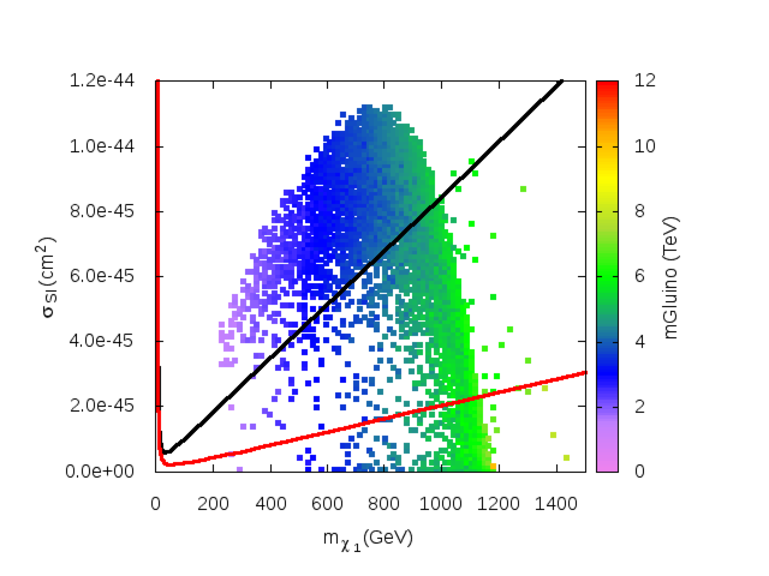
\includegraphics[width=0.45\textwidth]{ezssm_direct_detection}
    \hfill
    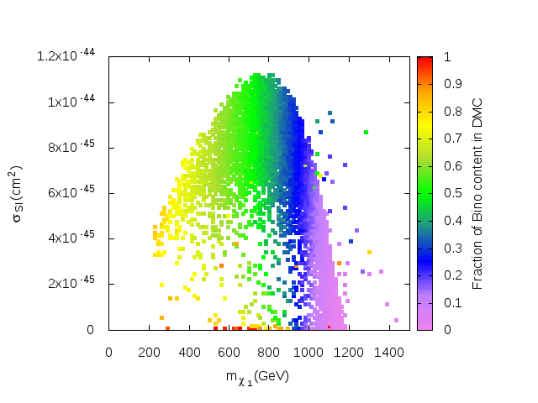
\includegraphics[width=0.45\textwidth]{ezssm_bino_fraction}
    \hfill
  \end{figure}
  \vspace*{-20pt}
  \begin{center}
    { \tiny [\href{http://arxiv.org/abs/1611.05966}{%
          arXiv:1611.05966}] }
  \end{center}
  \begin{itemize} \itemsep1em
  \item \alert{Note: none of these $Z_2$ symmetries commute with $E_6$}
  \end{itemize}
      {\tiny [2] J.~P.~Hall and S.~F.~King,
        \href{http://doi.org/10.1007/JHEP06(2011)006}{JHEP
          \textbf{1106}, 006 (20011)}
        (\href{http://arxiv.org/abs/1104.2259}{arXiv:1104.2259})}
\end{frame}

\section{The SE$_6$SSM}

\section{Results}

\section{Summary}

\begin{frame}
  \frametitle{Summary}
    \begin{center}
    \large Thank you for listening!
  \end{center}
\end{frame}

\end{document}
